% 附录 AI：惯性约束内爆与点火（v1.26.13 新增）
%
% 数值唯一来源：tools/calc/appAI_calc.py（只 print，不写文件）→ tools/calc/appAI_calc.txt。
%   本节凡标出数字的量都由该脚本复算；其余只能定性引用。
% 单位写法：数字与单位一律进数学模式（避免中文字符落进数学字体）；
%   温度用 keV 或 eV、面密度用 g/cm^2、压力用 Pa 并给出 Gbar/Mbar 换算。
% 口径：本附录的靶参数与附录 Y 的第 6 节是同一个点（燃料 2.82743 mg、rhoR = 3 g/cm^2、
%   rho = 200 g/cm^3、G = 160.033），只是把附录 Y 的 0-D 账展开成驱动、内爆、
%   稳定性、热斑与燃烧五段过程；增益与电厂账的分工见附录 U 与附录 Z。
% 版权口径：只借鉴结论、公式形式与题型；文字、数值、表格自拟并独立复算；
%   离线环境无法核验 DOI，故只给书名 / 作者 / 年份 / 卷期页。

\begin{figure}[htbp]
\centering
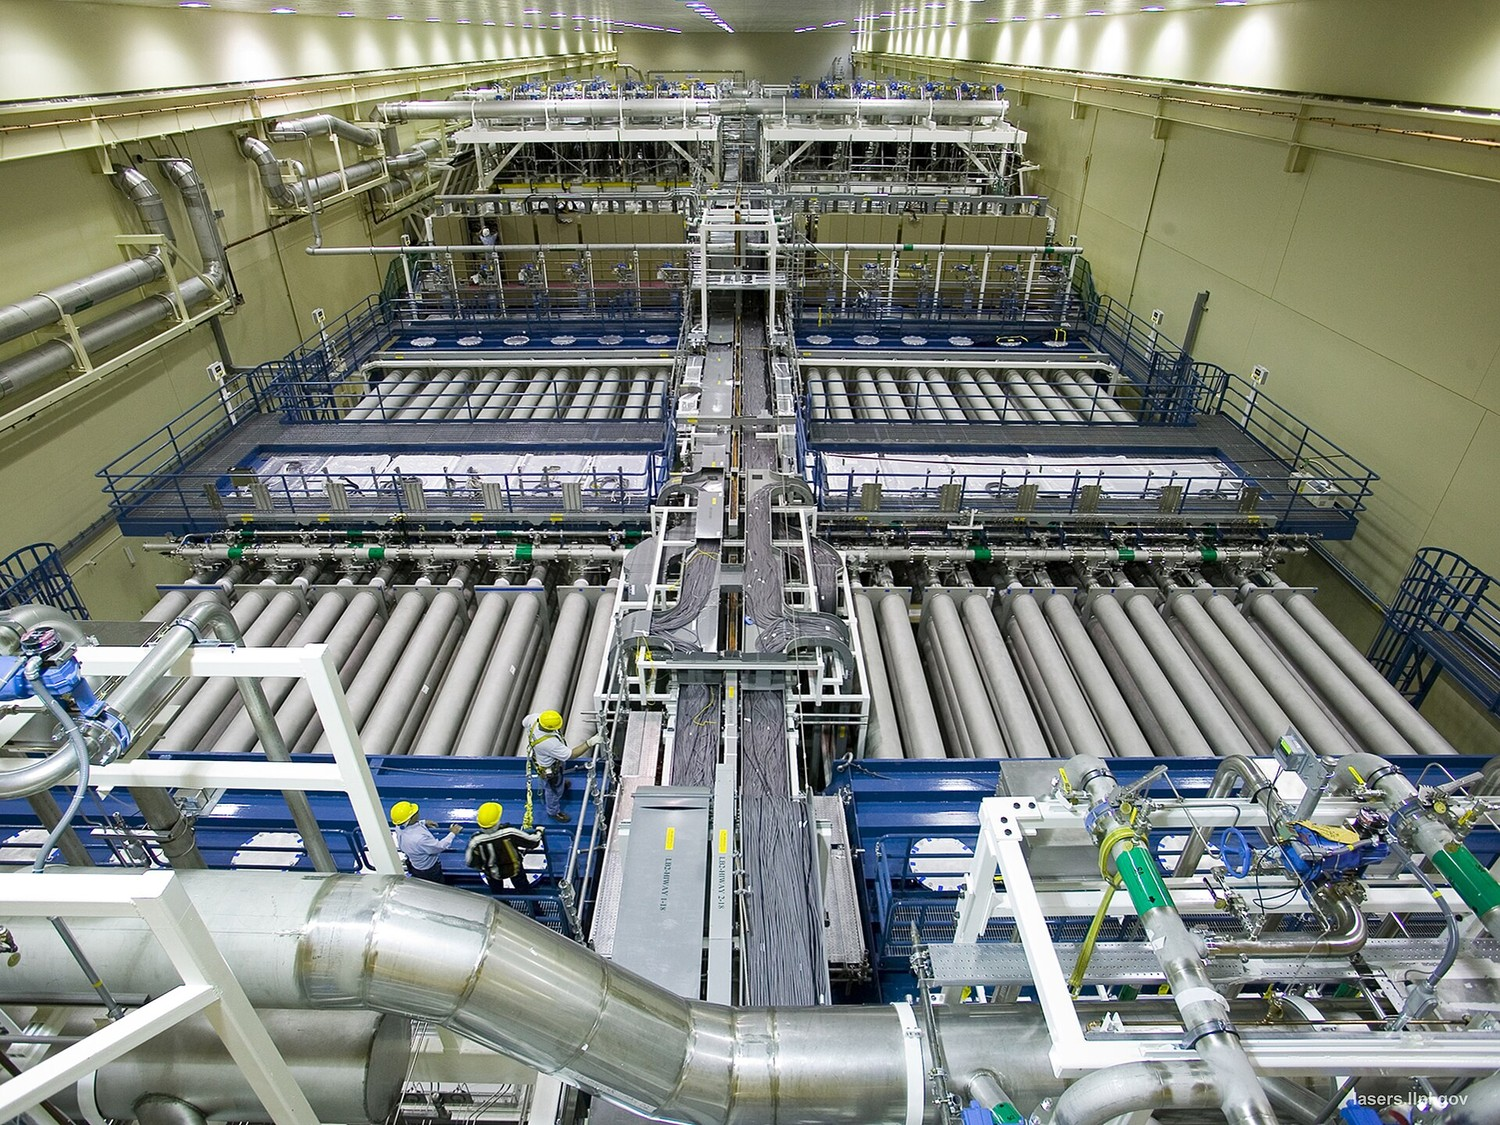
\includegraphics[width=0.78\textwidth]{../figures/nif_laser_bay.jpg}
\caption{驱动器的尺度：激光阵列。黑腔里的辐射温度不是凭空来的：几百束激光要在几十微米的目标上同时对准，每束的能量、脉宽与同步误差都直接进本章的驱动账。}
\label{fig:photo-appai2}
\figsource{Lawrence Livermore National Laboratory, Lawrence Livermore N，Public domain（Wikimedia Commons），链接见 figures/CREDITS.md。}
\end{figure}

\section{驱动：黑腔里的辐射温度}
\label{sec:app-ai-drive}

惯性约束的第一件事不是压缩，是\textbf{把能量送进去}。激光不能直接照在燃料上：
直接驱动的靶要面对激光的成丝与散射，于是主流方案把激光打进一个金壁小腔（
\textbf{黑腔}，hohlraum），先转成 X 射线，再由 X 射线均匀地烧蚀靶丸。这一步的
汇率是\textbf{转换效率} $\eta_{\mathrm{ce}}$，本附录取 $0.85$（声明值，量级）。

腔壁吸收 X 射线又再辐射，腔内建立起近似的黑体辐射场。壁面通量由能量守恒给出：
激光能量 $E_{\mathrm{drv}}$ 在脉宽 $\tau$ 内转成 X 射线，摊在腔壁上：

\begin{equation}
F_X = \frac{\eta_{\mathrm{ce}} E_{\mathrm{drv}}}{A_{\mathrm{hohl}}\, \tau}
= \sigma T_{\mathrm{rad}}^4,
\qquad
A_{\mathrm{hohl}} = 2\pi R L + 2\pi R^2 .
\label{eq:app-ai-flux}
\end{equation}

把 $E_{\mathrm{drv}} = 2.0$ MJ、$\eta_{\mathrm{ce}} = 0.85$、$\tau = 4.0$ ns、
$R = 1.5$ mm、$L = 5.0$ mm 代进去：$A_{\mathrm{hohl}} = 6.12611\times10^{-5}$ m$^2$
（$0.612611$ cm$^2$）、$E_X = 1.7$ MJ、$F_X = 6.93752\times10^{18}$ W m$^{-2}$，
于是

\begin{equation}
T_{\mathrm{rad}} = \left(\frac{F_X}{\sigma}\right)^{1/4}
= 3.32582\times10^{6}\ \mathrm{K} = 286.597\ \mathrm{eV},
\qquad
P_{\mathrm{rad}} = \frac{a T^4}{3},\quad a = \frac{4\sigma}{c}.
\label{eq:app-ai-prad}
\end{equation}

$286.597$ eV 听起来不吓人，但辐射压是 $P_{\mathrm{rad}} = 3.08548\times10^{10}$ Pa
（$0.308548$ Mbar），辐射能密度 $u = aT^4 = 9.25643\times10^{10}$ J m$^{-3}$。
真正说明问题的是\textbf{腔内储存的辐射能}：$u V = 3271.49$ J，只占 $E_X = 1.7$ MJ 的
千分之二。黑腔不是炉子，是\textbf{中转站}：X 射线一边产生一边被壁吸收、再辐射、
再被靶丸吸收，能量始终在流动。

\begin{table}[htbp]
\centering
\small
\begin{tabular}{p{3.4cm}p{3.0cm}p{3.4cm}p{3.6cm}}
\toprule
量 & 表达式 & 数值 & 说明 \\
\midrule
激光能量 & $E_{\mathrm{drv}}$ & $2.0\ \mathrm{MJ}$ & 3$\omega$（$0.35\ \mu$m）声明值 \\
转换效率 & $\eta_{\mathrm{ce}}$ & $0.85$ & 激光 $\to$ X 射线，声明值 \\
X 射线能量 & $\eta_{\mathrm{ce}}E_{\mathrm{drv}}$ & $1.7\ \mathrm{MJ}$ & 式 \eqref{eq:app-ai-flux} \\
腔壁面积 & $A_{\mathrm{hohl}}$ & $6.12611\times10^{-5}\ \mathrm{m^2}$ & 圆柱侧面积加两个端面 \\
壁面通量 & $F_X$ & $6.93752\times10^{18}\ \mathrm{W\,m^{-2}}$ & 与 $\sigma T^4$ 一致 \\
辐射温度 & $T_{\mathrm{rad}}$ & $286.597\ \mathrm{eV}$ & 黑腔的「工作温度」 \\
辐射压 & $aT^4/3$ & $0.308548\ \mathrm{Mbar}$ & 式 \eqref{eq:app-ai-prad} \\
腔内辐射能 & $uV$ & $3271.49\ \mathrm{J}$ & 只占 $E_X$ 的 $0.19\%$ \\
\bottomrule
\end{tabular}
\caption{黑腔与辐射场的账。黑腔的温度由\emph{通量}决定，不由\emph{储存的能量}决定：
这就是为什么 $T_{\mathrm{rad}}$ 只按 $E^{1/4}$ 变。}
\label{tab:app-ai-drive}
\end{table}

\begin{tip}{黑腔不是炉子，是能量中转站}{tip-app-ai-hohlraum}
炉子靠储存的热量工作，黑腔靠\emph{通量}工作。腔内储存的辐射能只有几千焦，
远小于驱动激光的兆焦量级；真正决定烧蚀压的是壁面通量 $\sigma T^4$。
把 $T_{\mathrm{rad}}$ 当成「腔里的温度」会算错量级，把它当成「通量的等效温度」才对。
\end{tip}

\textbf{出处：}本文的间接驱动与黑腔图像、转换效率与辐射温度的口径参照
Lindl \emph{Physics of Plasmas}（1995，第 2 卷，3933 页）与 Lindl 等
\emph{Physics of Plasmas}（2004，第 11 卷，339 页）；黑腔能量平衡的形式参照
Atzeni \& Meyer-ter-Vehn \emph{The Physics of Inertial Fusion}（2004，第 10 章）。
本节凡标出数字的量都由 \texttt{tools/\allowbreak{}calc/\allowbreak{}appAI\_calc.py} 复算。

\section{内爆：火箭模型与滞止}
\label{sec:app-ai-implosion}

X 射线烧蚀靶丸外壳，外壳向外喷出的等离子体把剩下的壳层向内推——这就是
\textbf{火箭}。动量守恒给出火箭方程：把烧蚀层当作燃料，把剩下的靶丸当作载荷，

\begin{equation}
v_{\mathrm{imp}} = v_{\mathrm{ex}} \ln\frac{m_0}{m_f},
\label{eq:app-ai-rocket}
\end{equation}

其中 $v_{\mathrm{ex}}$ 是烧蚀排出速度（本附录取 $330$ km/s，声明为量级值），
$m_0$ 是靶丸初始质量，$m_f$ 是剩下的载荷质量。本附录的靶：
燃料冰球半径 $R_{\mathrm{ice}} = 1.38331$ mm、质量 $2.82743$ mg，
外面包 $150\ \mu$m 的 CH 烧蚀层（$m_{\mathrm{abl}} = 4.21285$ mg），
于是 $m_0 = 7.04028$ mg、$m_0/m_f = 2.48999$、$\ln(m_0/m_f) = 0.912279$，

\begin{equation}
v_{\mathrm{imp}} = 301.052\ \mathrm{km\,s^{-1}},
\qquad
E_{\mathrm{kin}} = \tfrac12 m_f v_{\mathrm{imp}}^2 = 128.128\ \mathrm{kJ},
\qquad
\frac{E_{\mathrm{kin}}}{E_{\mathrm{drv}}} = 6.40642\%.
\label{eq:app-ai-ekin}
\end{equation}

六兆焦的驱动能量里只有 $128$ kJ 变成内爆动能——这个 $6.4\%$ 就是\textbf{流体力学效率}，
是惯性约束最硬的约束之一。内爆时间 $t_{\mathrm{imp}} = R_{\mathrm{ice}}/v_{\mathrm{imp}}
= 4.59493$ ns，与驱动脉宽同量级；平均加速度
$a = 3.27591\times10^{13}$ m s$^{-2}$（$3.34277\times10^{12}$ 倍地表重力）。
滞止时壳层的动压是

\begin{equation}
P_{\mathrm{stag}} \sim \rho v_{\mathrm{imp}}^2 = 1.81265\times10^{16}\ \mathrm{Pa}
= 181.265\ \mathrm{Gbar},
\label{eq:app-ai-stag}
\end{equation}

比太阳中心的压力还高几个量级。燃料被压到 $R_f = 150\ \mu$m、
$\rho = 200$ g cm$^{-3}$：半径压缩比 $9.2221$、密度压缩比 $784.314$、
面密度 $\rho R = 3$ g cm$^{-2}$——这正是附录 Y 第 6 节那个 0-D 工作点，
现在它有了过程。

\begin{table}[htbp]
\centering
\small
\begin{tabular}{p{3.4cm}p{2.8cm}p{3.2cm}p{4.0cm}}
\toprule
量 & 表达式 & 数值 & 说明 \\
\midrule
排出速度 & $v_{\mathrm{ex}}$ & $330\ \mathrm{km\,s^{-1}}$ & 声明量级值 \\
质量比 & $m_0/m_f$ & $2.48999$ & 烧蚀掉 $59.8\%$ 的初始质量 \\
内爆速度 & 式 \eqref{eq:app-ai-rocket} & $301.052\ \mathrm{km\,s^{-1}}$ & 设计目标 $300$ 量级 \\
内爆动能 & $\frac12 m_f v^2$ & $128.128\ \mathrm{kJ}$ & 式 \eqref{eq:app-ai-ekin} \\
流体力学效率 & $E_{\mathrm{kin}}/E_{\mathrm{drv}}$ & $6.40642\%$ & 兆焦驱动只留千焦动能 \\
内爆时间 & $R_{\mathrm{ice}}/v_{\mathrm{imp}}$ & $4.59493\ \mathrm{ns}$ & 与脉宽同量级 \\
平均加速度 & $v^2/2R$ & $3.27591\times10^{13}\ \mathrm{m\,s^{-2}}$ & $3.34277\times10^{12}\,g_0$ \\
滞止动压 & $\rho v^2$ & $181.265\ \mathrm{Gbar}$ & 式 \eqref{eq:app-ai-stag} \\
压缩结果 & $R_f$, $\rho$, $\rho R$ & $150\ \mu$m, $200$ g cm$^{-3}$, $3$ g cm$^{-2}$ & 与附录 Y 同点 \\
\bottomrule
\end{tabular}
\caption{内爆账。质量比决定速度，速度平方决定动能：这就是为什么烧蚀层厚度
与排出速度是设计里最敏感的两个旋钮。}
\label{tab:app-ai-implosion}
\end{table}

\begin{tip}{质量比决定内爆速度}{tip-app-ai-rocket}
火箭方程里没有压强、没有温度、没有烧蚀率——只有质量比与排出速度。
压强决定的是\emph{能不能}在给定时间里烧蚀掉那么多质量，而不是直接决定速度。
把烧蚀层加厚会提高质量比、提高 $v_{\mathrm{imp}}$，但要多花驱动能量：
这是一个必须一起算的权衡（见练习 2）。
\end{tip}

\textbf{出处：}本文的火箭模型与内爆参数化参照 Atzeni \& Meyer-ter-Vehn
\emph{The Physics of Inertial Fusion}（2004，第 7 章）；惯性约束聚变的原始构想见
Nuckolls 等 \emph{Nature}（1972，第 239 卷，139 页）；滞止动压的量级口径参照
Lindl \emph{Physics of Plasmas}（1995，第 2 卷，3933 页）。
本节凡标出数字的量都由 \texttt{tools/\allowbreak{}calc/\allowbreak{}appAI\_calc.py} 复算。

\section{绝热与熵：为什么压缩要冷}
\label{sec:app-ai-adiabat}

燃料被压缩 $784$ 倍，为什么温度不跟着涨 $784^{2/3}$ 倍？因为压缩分成两种：
\textbf{等熵压缩}（慢、可逆、$P \propto \rho^{5/3}$）与\textbf{激波压缩}
（不可逆、熵增）。设计的目标是尽量等熵，用一个无量纲数衡量：

\begin{equation}
\alpha_{\mathrm{ad}} \equiv \frac{P_{\mathrm{th}}}{P_F},
\qquad
P_F = \frac{(3\pi^2)^{2/3}\hbar^2}{5 m_e} n_e^{5/3},
\label{eq:app-ai-fermi}
\end{equation}

即热压与\textbf{费米压}（电子简并压）之比。$\alpha_{\mathrm{ad}} \sim 1$ 表示
燃料已经简并，压力主要来自泡利原理而不是温度——这正是「冷压缩」的意思：

\begin{equation}
P_F(\rho = 200\ \mathrm{g\,cm^{-3}}) = 1.49065\times10^{15}\ \mathrm{Pa}
= 14.9065\ \mathrm{Gbar},
\qquad
P_{\mathrm{th}}(100\ \mathrm{eV}) = 7.71883\times10^{14}\ \mathrm{Pa},
\label{eq:app-ai-adiabat}
\end{equation}

于是冷燃料 $\alpha_{\mathrm{ad}} = 0.517816$——它已经被简并压撑住，温度不是主要压力来源。
热斑完全相反：$\rho = 30$ g cm$^{-3}$ 时 $P_F = 6.3124\times10^{13}$ Pa，
而 $5$ keV 的热压是 $5.78912\times10^{15}$ Pa，$\alpha_{\mathrm{ad}} = 91.7103$——
热斑是理想气体，必须靠惯性约束住。

激波是熵的敌人。强激波（$\gamma = 5/3$）的压缩比上限是

\begin{equation}
\frac{\rho_2}{\rho_1} = \frac{\gamma+1}{\gamma-1} = 4,
\label{eq:app-ai-shock}
\end{equation}

单靠一道激波只能压四倍；再压就要靠等熵的持续做功。这解释了为什么点火靶不用
一道强激波把燃料压到 $200$ g cm$^{-3}$：那会产生太多熵，把燃料变成难以压缩的热气体。
实际设计用\textbf{一串精心定时的激波}在燃料里会聚，使每一道激波都尽量弱、总熵增最小。

\begin{table}[htbp]
\centering
\small
\begin{tabular}{p{4.2cm}p{3.2cm}p{3.0cm}p{3.0cm}}
\toprule
量 & 表达式 & 数值 & 说明 \\
\midrule
压缩燃料电子密度 & $n_e$ & $4.81771\times10^{31}\ \mathrm{m^{-3}}$ & $\rho = 200$ g cm$^{-3}$ \\
费米压 & $P_F$ & $14.9065\ \mathrm{Gbar}$ & 式 \eqref{eq:app-ai-fermi} \\
冷燃料热压 & $P_{\mathrm{th}}(100\ \mathrm{eV})$ & $7.71883\times10^{14}\ \mathrm{Pa}$ & 简并压主导 \\
冷燃料绝热因子 & $\alpha_{\mathrm{ad}}$ & $0.517816$ & 小于一：已简并 \\
热斑费米压 & $P_F(30\ \mathrm{g\,cm^{-3}})$ & $6.3124\times10^{13}\ \mathrm{Pa}$ & 密度低，简并弱 \\
热斑热压 & $P_{\mathrm{th}}(5\ \mathrm{keV})$ & $5.78912\times10^{15}\ \mathrm{Pa}$ & 理想气体 \\
热斑绝热因子 & $\alpha_{\mathrm{ad}}$ & $91.7103$ & 远大于一 \\
强激波压缩比上限 & $(\gamma+1)/(\gamma-1)$ & $4$ & 式 \eqref{eq:app-ai-shock} \\
\bottomrule
\end{tabular}
\caption{绝热因子账。同一个词 $\alpha_{\mathrm{ad}}$ 在冷燃料与热斑里差两个数量级，
这正是「冷压缩、热点火」的分工。}
\label{tab:app-ai-adiabat}
\end{table}

\begin{tip}{温度不是压缩的障碍，熵才是}{tip-app-ai-adiabat}
初学者常以为「压缩会让燃料变热，所以压不下去」。真正拦住压缩的是\emph{熵}：
熵越高，同样密度下压力越大。简并的冷燃料 $\alpha_{\mathrm{ad}} < 1$，
可以压到几百克每立方厘米；一旦激波把熵抬起来，同样的压缩就要付出高得多的压力代价。
\end{tip}

\textbf{出处：}本文的简并压与绝热压缩图像参照 Atzeni \& Meyer-ter-Vehn
\emph{The Physics of Inertial Fusion}（2004，第 3 章）；激波关系与熵增的经典处理见
Zel'dovich \& Raizer \emph{Physics of Shock Waves and High-Temperature Hydrodynamic
Phenomena}（1966 初版 / 2002 再版，第 1--2 章）；脉冲整形与激波定时的讨论参照
Lindl \emph{Physics of Plasmas}（1995，第 2 卷，3933 页）。
本节凡标出数字的量都由 \texttt{tools/\allowbreak{}calc/\allowbreak{}appAI\_calc.py} 复算。

\section{流体不稳定性：瑞利--泰勒与烧蚀稳定化}
\label{sec:app-ai-rt}

内爆是一层重流体（壳层）被轻流体（烧蚀等离子体）推着加速——这正是
\textbf{瑞利--泰勒不稳定性}（RT）的经典位形：加速度指向重流体时，界面上的扰动
指数增长，

\begin{equation}
\gamma_{\mathrm{RT}} = \sqrt{A_T k g},
\qquad
k = \frac{2\pi}{\lambda},
\label{eq:app-ai-rt}
\end{equation}

其中 $A_T$ 是阿特伍德数（本附录取 $0.85$，声明值）、$g$ 是加速度、
$\lambda$ 是扰动波长。取 $g = 1.0\times10^{14}$ m s$^{-2}$（与
$a = 3.27591\times10^{13}$ m s$^{-2}$ 同量级，声明取值），
$\lambda = 10\ \mu$m 的短波扰动：

\begin{equation}
k = 628319\ \mathrm{m^{-1}},
\qquad
\gamma_{\mathrm{RT}} = 7.30801\times10^{9}\ \mathrm{s^{-1}},
\qquad
\tau = \frac{1}{\gamma} = 0.136836\ \mathrm{ns}.
\label{eq:app-ai-rtabl}
\end{equation}

不加任何稳定化，扰动在 $4.59493$ ns 的内爆时间里会放大
$e^{33.5798} \approx 4\times10^{14}$ 倍——足以把靶丸撕碎。真实靶没被撕碎，
靠的是\textbf{烧蚀稳定化}：烧蚀前沿以 $v_{\mathrm{abl}}$ 扫过界面，把短波扰动
（波长小于烧蚀层厚度量级）对流走：

\begin{equation}
\gamma^2 = A_T k g - k^2 v_{\mathrm{abl}}^2 ,
\qquad
k_c = \frac{A_T g}{v_{\mathrm{abl}}^2},
\qquad
k_{\max} = \frac{k_c}{2}.
\label{eq:app-ai-cutoff}
\end{equation}

取 $v_{\mathrm{abl}} = 3.0\times10^{4}$ m s$^{-1}$（声明值）：
$k_c = 94444.4$ m$^{-1}$（截止波长 $\lambda_c = 66.5278\ \mu$m）、
最不稳定波长 $\lambda_{\max} = 133.056\ \mu$m、
$\gamma_{\max} = 1.41667\times10^{9}$ s$^{-1}$，内爆期间的最大放大倍数降到

\begin{equation}
N_{e} = \gamma_{\max} t_{\mathrm{imp}} = 6.50949 ,
\qquad
\delta_f = \delta_0 e^{N_e}.
\label{eq:app-ai-efold}
\end{equation}

$\delta_0 = 20$ nm 的种子会长到 $\delta_f = 13.4297\ \mu$m，
占最终半径 $150\ \mu$m 的 $8.95311\%$——还在可接受范围，但余量不大。
反过来问：若要求末期扰动不超过 $5\ \mu$m，则种子必须
$\delta_0 \le 7.4462$ nm。这就是为什么靶丸表面粗糙度要控制在纳米量级，
也是为什么内爆的加速度、烧蚀速度与表面质量必须一起设计。

\begin{table}[htbp]
\centering
\small
\begin{tabular}{p{3.6cm}p{3.2cm}p{3.0cm}p{3.2cm}}
\toprule
量 & 表达式 & 数值 & 说明 \\
\midrule
扰动波数 & $2\pi/\lambda$ & $628319\ \mathrm{m^{-1}}$ & $\lambda = 10\ \mu$m \\
无稳定化增长率 & $\sqrt{A_T k g}$ & $7.30801\times10^{9}\ \mathrm{s^{-1}}$ & 式 \eqref{eq:app-ai-rt} \\
无稳定化时间 & $1/\gamma$ & $0.136836\ \mathrm{ns}$ & 远小于内爆时间 \\
无稳定化放大 & $\gamma t_{\mathrm{imp}}$ & $33.5798$ & 约 $4\times10^{14}$ 倍 \\
截止波数 & $A_T g/v_{\mathrm{abl}}^2$ & $94444.4\ \mathrm{m^{-1}}$ & 式 \eqref{eq:app-ai-cutoff} \\
截止波长 & $2\pi/k_c$ & $66.5278\ \mu$m & 短于此波长被对流稳定 \\
最不稳定波长 & $2\pi/k_{\max}$ & $133.056\ \mu$m & $k_{\max} = k_c/2$ \\
最大增长率 & $\sqrt{A_T k_c g}/2$ & $1.41667\times10^{9}\ \mathrm{s^{-1}}$ & 降低 $5.16$ 倍 \\
最大放大倍数 & $\gamma_{\max}t_{\mathrm{imp}}$ & $6.50949$ & 式 \eqref{eq:app-ai-efold} \\
种子 $20$ nm 的末期幅度 & $\delta_0 e^{N_e}$ & $13.4297\ \mu$m & 占 $R_f$ 的 $8.95311\%$ \\
末期 $5\ \mu$m 对应的种子 & $\delta_0$ & $\le 7.4462\ \mathrm{nm}$ & 表面粗糙度指标 \\
\bottomrule
\end{tabular}
\caption{瑞利--泰勒账。稳定化把放大倍数从 $10^{14}$ 压到 $e^{6.51} \approx 673$，
但代价是只有长波被压住、短波被对流扫走——总放大倍数仍必须逐位管理。}
\label{tab:app-ai-rt}
\end{table}

\begin{tip}{不稳定性要按 e 倍增长数管理}{tip-app-ai-rt}
「有没有不稳定性」是个错问题：瑞利--泰勒在任何加速界面上都存在。
工程上可控的量是\emph{e 倍增长数} $N_e$ 与\emph{末期幅度}/\emph{允许幅度}之比。
把这两个数算出来，才能判断表面粗糙度、激波定时与掺杂层厚度的余量；
只讨论「稳定不稳定」不会给出任何设计约束。
\end{tip}

\textbf{出处：}本文的瑞利--泰勒不稳定性经典处理见 Rayleigh \emph{Proceedings of the
London Mathematical Society}（1883，第 14 卷，170 页）与 Taylor \emph{Proceedings of
the Royal Society A}（1950，第 201 卷，192 页）；界面冲击加速的对应结果见
Richtmyer \emph{Communications on Pure and Applied Mathematics}（1960，第 13 卷，
297 页）与 Meshkov（1969，第 4 卷，101 页）；烧蚀稳定化与内爆不稳定性综述参照
Kilkenny 等 \emph{Physics of Plasmas}（1994，第 1 卷，1379 页）与 Atzeni \&
Meyer-ter-Vehn \emph{The Physics of Inertial Fusion}（2004，第 8 章）。
本节凡标出数字的量都由 \texttt{tools/\allowbreak{}calc/\allowbreak{}appAI\_calc.py} 复算。

\begin{figure}[htbp]
\centering
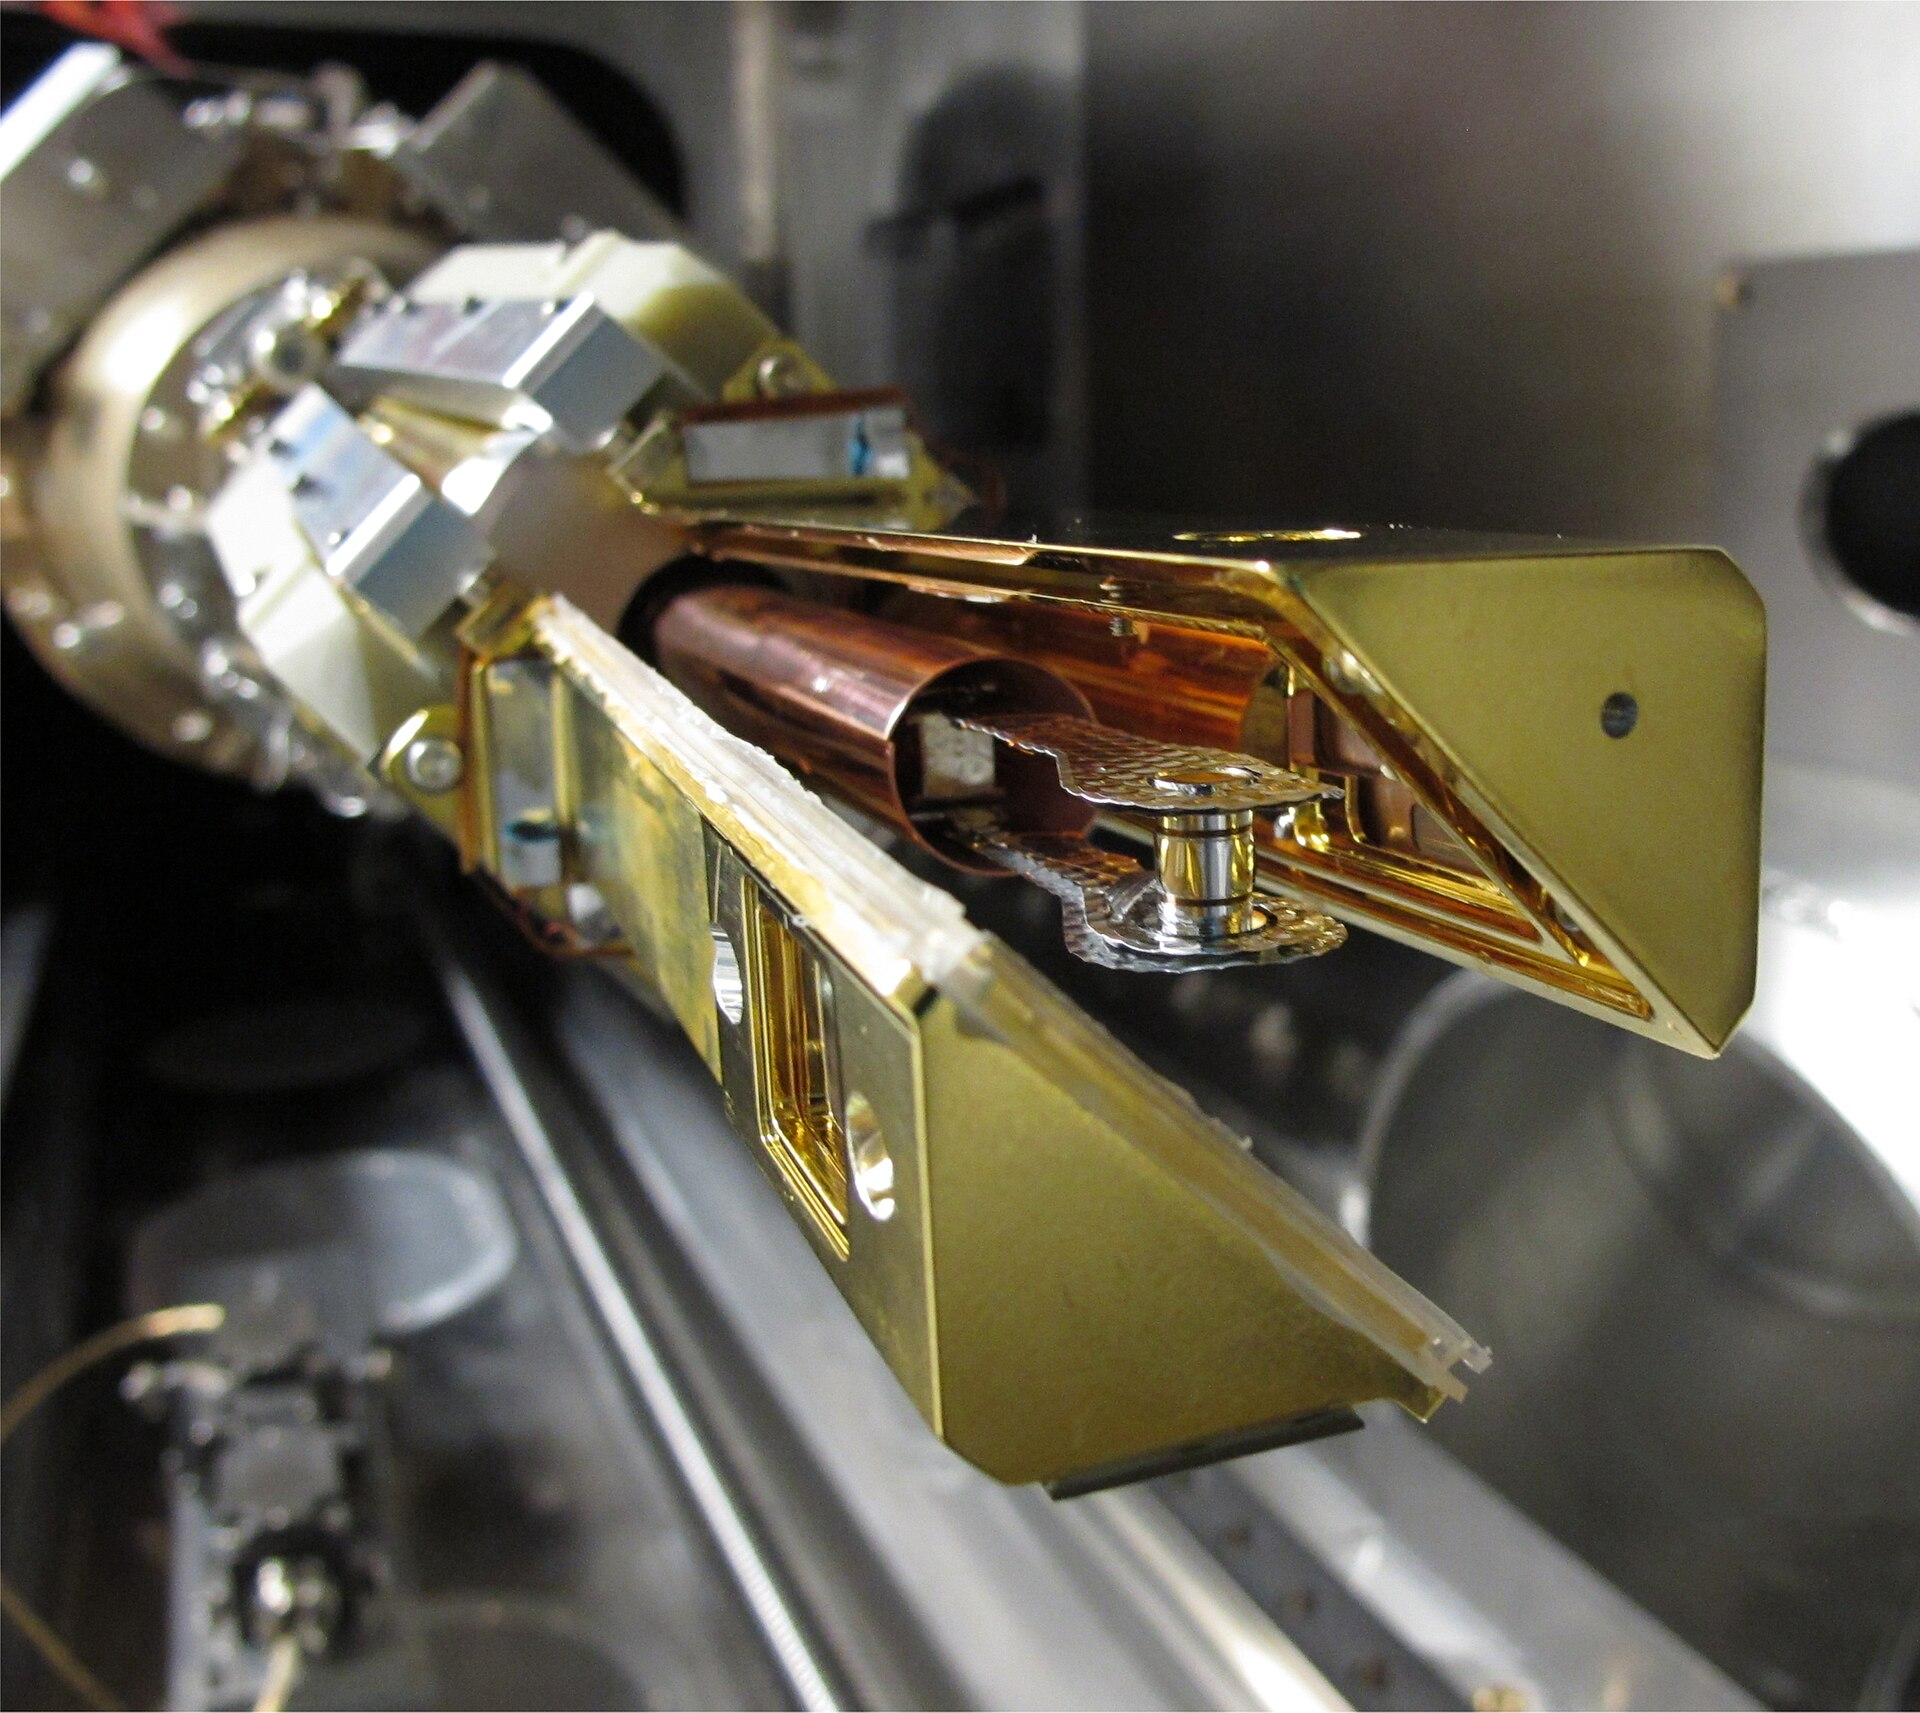
\includegraphics[width=0.78\textwidth]{../figures/ai_nif_target_assembly.jpg}
\caption{美国国家点火装置的靶装配体：金色锥体是黑腔（hohlraum），中间那颗毫米级小丸就是燃料靶丸，整件东西装在同轴定位臂上送进靶室中心，对准误差要小于本节算的数十微米级。}
\label{fig:photo-appai3}
\figsource{Lawrence Livermore National Security, LLC，CC BY-SA 3.0（Wikimedia Commons）}
\end{figure}

\section{热斑与点火：自加热怎样跑赢轫致损失}
\label{sec:app-ai-ignition}

压缩到最后，中心形成一个高温低密的\textbf{热斑}：本附录取
$r = 40\ \mu$m、$\rho = 30$ g cm$^{-3}$、$T = 5$ keV（声明设计点）。
热斑的第一个账是面密度：

\begin{equation}
\rho R_{\mathrm{hot}} = 0.12\ \mathrm{g\,cm^{-2}},
\qquad
E_{\mathrm{hot}} = 2327.94\ \mathrm{J},
\qquad
P = 5.78912\times10^{15}\ \mathrm{Pa} = 57.8912\ \mathrm{Gbar}.
\label{eq:app-ai-hotspot}
\end{equation}

$\alpha$ 粒子在 DT 里的射程对应 $\rho R \approx 0.3$ g cm$^{-2}$（声明值），
在 $200$ g cm$^{-3}$ 的冷燃料里约 $15\ \mu$m、在热斑密度里约 $100\ \mu$m。
热斑的 $\rho R_{\mathrm{hot}} = 0.12$ g cm$^{-2}$ \textbf{只有阈值的 $2.5$ 分之一}——
这是一个刻意的设计点：热斑不必自己把 $\alpha$ 全部拦住，它只要点燃，
剩下的 $\alpha$ 会在外面那层 $\rho R = 3$ g cm$^{-2}$ 的冷燃料里沉积。

热斑靠声速散开，滞止时间

\begin{equation}
\tau_{\mathrm{dwell}} = \frac{r}{c_s} = 64.3872\ \mathrm{ps},
\qquad
c_s = \sqrt{\frac{2 k T}{m_i}} = 621.242\ \mathrm{km\,s^{-1}},
\label{eq:app-ai-dwell}
\end{equation}

燃烧的反应率用 $\langle\sigma v\rangle(5\ \mathrm{keV}) = 2.75\times10^{-23}$ m$^3$ s$^{-1}$
（声明值，DT）：

\begin{equation}
\begin{aligned}
P_\alpha &= \frac{n_D n_T}{1+\delta_{DT}} \langle\sigma v\rangle E_\alpha
= 2.01333\times10^{26}\ \mathrm{W\,m^{-3}},\\
P_{\mathrm{br}} &= 6.24074\times10^{25}\ \mathrm{W\,m^{-3}},\qquad
\frac{P_\alpha}{P_{\mathrm{br}}} = 3.22611 .
\end{aligned}
\label{eq:app-ai-alpha}
\end{equation}

轫致辐射功率沿用附录 X 的口径（$Z_{\mathrm{eff}}$ 与相对论修正都在那里算过）：

\begin{equation}
P_{\mathrm{br}} \propto n_e^2 Z_{\mathrm{eff}} \sqrt{T},
\label{eq:app-ai-brems}
\end{equation}

一个滞止时间里 $\alpha$ 沉积 $3475.23$ J（$=1.49283\,E_{\mathrm{hot}}$）、
轫致损失 $1077.22$ J：自加热已经跑赢损失，热斑能自我维持。
但这个结论对温度很敏感：

\begin{equation}
\begin{aligned}
\frac{P_\alpha}{P_{\mathrm{br}}}(T) &= 0.288552\ (1\ \mathrm{keV}),\;
0.816149\ (2),\; 1.49936\ (3),\; 2.30842\ (4),\\
&\quad 3.22611\ (5),\; 5.34406\ (7),\; 9.12482\ (10).
\end{aligned}
\label{eq:app-ai-range}
\end{equation}

按本附录采用的 $\langle\sigma v\rangle$ 拟合，两条曲线在 $2.4$ keV 附近交叉；
文献报道的理想点火温度约 $4.3$ keV。两者差在低 $T$ 端的反应率拟合上
（本书用的 $\langle\sigma v\rangle \approx 1.1\times10^{-24}T^2$ 在低 $T$ 偏高），
以文献值为准。这条曲线的意义是：\textbf{点火不是把温度推到某个数，
是让自加热在热斑散开之前超过损失}。

\begin{table}[htbp]
\centering
\small
\begin{tabular}{p{4.0cm}p{3.0cm}p{3.0cm}p{3.0cm}}
\toprule
量 & 表达式 & 数值 & 说明 \\
\midrule
热斑面密度 & $\rho r$ & $0.12\ \mathrm{g\,cm^{-2}}$ & 阈值的 $2.5$ 分之一 \\
热斑能量 & $P V$ & $2327.94\ \mathrm{J}$ & 式 \eqref{eq:app-ai-hotspot} \\
热斑压力 & $n k T$ & $57.8912\ \mathrm{Gbar}$ & 惯性约束 \\
声速 & $\sqrt{2kT/m_i}$ & $621.242\ \mathrm{km\,s^{-1}}$ & 式 \eqref{eq:app-ai-dwell} \\
滞止时间 & $r/c_s$ & $64.3872\ \mathrm{ps}$ & 自加热的时间窗口 \\
$\alpha$ 功率密度 & 式 \eqref{eq:app-ai-alpha} & $2.01333\times10^{26}\ \mathrm{W\,m^{-3}}$ & $5$ keV，DT \\
轫致功率密度 & 式 \eqref{eq:app-ai-brems} & $6.24074\times10^{25}\ \mathrm{W\,m^{-3}}$ & 附录 X 口径 \\
自加热/损失 & $P_\alpha/P_{\mathrm{br}}$ & $3.22611$ & 已跑赢 \\
一个滞止时间 $\alpha$ 沉积 & $P_\alpha V \tau$ & $3475.23\ \mathrm{J}$ & $1.49283\,E_{\mathrm{hot}}$ \\
一个滞止时间轫致损失 & $P_{\mathrm{br}} V \tau$ & $1077.22\ \mathrm{J}$ & 约一半热斑能量 \\
模型交叉温度 & $P_\alpha = P_{\mathrm{br}}$ & 约 $2.4\ \mathrm{keV}$ & 文献理想值 $4.3$ keV \\
$\alpha$ 射程 & $\rho R = 0.3\ \mathrm{g\,cm^{-2}}$ & $15\ \mu$m ($200$ g cm$^{-3}$) & 热斑外由冷燃料拦住 \\
\bottomrule
\end{tabular}
\caption{热斑账。点火的关键不是「热斑够大」，而是「$\alpha$ 在热斑散开前
留下足够的能量，剩下的被外面的冷燃料吸收」。}
\label{tab:app-ai-ignition}
\end{table}

\begin{tip}{点火是自加热跑赢损失}{tip-app-ai-ignition}
温度、密度、面密度都不是点火的判据本身：判据是 $\alpha$ 自加热率与
轫致损失率（加上膨胀损失）的相对大小，而且必须在滞止时间之内成立。
把 $2.4$ keV 与文献 $4.3$ keV 的差别记住：判据的形式比判据上的具体数字更可靠。
\end{tip}

\textbf{出处：}本文的热斑与点火图像、$\alpha$ 自加热判据参照 Betti \& Hurricane
\emph{Nature Physics}（2016，第 12 卷，435 页）与 Hurricane 等 \emph{Nature}
（2014，第 506 卷，343 页）；DT 反应率数据见 Bosch \& Hale \emph{Nuclear Fusion}
（1992，第 32 卷，611 页）；轫致损失的公式与数值口径与附录 X 一致，另见
Wesson \emph{Tokamaks}（第 4 版，2011，第 14 章）。本节凡标出数字的量都由
\texttt{tools/\allowbreak{}calc/\allowbreak{}appAI\_calc.py} 复算。

\section{燃烧与增益：把三本账合起来}
\label{sec:app-ai-burn}

点火之后是燃烧。燃烧持续的时间由燃料半径与声速给出：

\begin{equation}
t_{\mathrm{burn}} = \frac{R_f}{c_s} = 0.241452\ \mathrm{ns},
\qquad
E_{\mathrm{fus}} = f\, m_{\mathrm{DT}}\, q_{\mathrm{DT}},
\label{eq:app-ai-burn}
\end{equation}

其中 $q_{\mathrm{DT}} = 3.396\times10^{14}$ J kg$^{-1}$ 是 DT 的比能，
燃耗份额用面密度拟合 $f = \rho R/(\rho R + 6\ \mathrm{g\,cm^{-2}})$：

\begin{equation}
f = \frac{3}{3+6} = 33.3333\%,
\qquad
E_{\mathrm{fus}} = 960.195\ \mathrm{MJ},
\qquad
E_{\mathrm{burn}} = 320.065\ \mathrm{MJ},
\label{eq:app-ai-gain}
\end{equation}

这里 $E_{\mathrm{burn}}$ 只是 $\alpha$ 带走的那部分（$E_{\mathrm{fus}}/3$ 左右，
本附录按 $E_\alpha = 63.66$ MJ、份额 $19.89\%$ 计入燃烧账）。靶增益与墙插增益：

\begin{equation}
G = \frac{E_{\mathrm{burn}}}{E_{\mathrm{drv}}} = 160.033,
\qquad
G_{\mathrm{wall}} = \eta_{\mathrm{drv}} G = 16.0033 \quad (\eta_{\mathrm{drv}} = 10\%),
\label{eq:app-ai-wall}
\end{equation}

\begin{equation}
\frac{E_\alpha}{E_{\mathrm{burn}}} = 19.89\%,
\qquad
\frac{E_{\mathrm{kin}}}{E_{\mathrm{drv}}} = 6.40642\%,
\qquad
\frac{E_{\mathrm{burn}}}{E_{\mathrm{kin}}} = 2498.0 .
\label{eq:app-ai-frac}
\end{equation}

最后一行是本附录最重要的一句话：\textbf{内爆动能只有 $128$ kJ，
而燃烧放能 $320$ MJ——放大了约两千五百倍}。惯性约束之所以值得做，
就是因为它用「压缩」这个小输入撬动「聚变」这个大输出；代价是每一步都要
在纳秒尺度上精确到位。

文献对照（文献级，只作对照不作断言）：美国国家点火装置在 2022 年 12 月
首次实现靶增益大于一，输入激光能量 $2.05$ MJ、聚变产额约 $3.15$ MJ，
对应靶增益约 $1.54$。本附录的 $G = 160.033$ 是\textbf{设计点}，
不是已实现的实验结果；两者相差两个数量级，这个差距正是当前 ICF 研究的全部内容。

\begin{table}[htbp]
\centering
\small
\begin{tabular}{p{4.0cm}p{3.0cm}p{3.0cm}p{3.0cm}}
\toprule
量 & 表达式 & 数值 & 说明 \\
\midrule
燃烧时间 & $R_f/c_s$ & $0.241452\ \mathrm{ns}$ & 式 \eqref{eq:app-ai-burn} \\
燃耗份额 & $\rho R/(\rho R+6)$ & $33.3333\%$ & 只烧掉三分之一 \\
聚变能 & $f m q$ & $960.195\ \mathrm{MJ}$ & 与附录 Y 一致 \\
$\alpha$ 能量 & $E_{\mathrm{fus}}/3$ 量级 & $63.66\ \mathrm{MJ}$ & 份额 $19.89\%$ \\
燃烧放能 & $\eta_\alpha E_{\mathrm{fus}}$ & $320.065\ \mathrm{MJ}$ & 式 \eqref{eq:app-ai-gain} \\
内爆动能 & 式 \eqref{eq:app-ai-ekin} & $128.128\ \mathrm{kJ}$ & 输入 \\
放大倍数 & $E_{\mathrm{burn}}/E_{\mathrm{kin}}$ & $2498.0$ & 压缩撬动聚变 \\
靶增益 & $E_{\mathrm{burn}}/E_{\mathrm{drv}}$ & $160.033$ & 式 \eqref{eq:app-ai-wall} \\
墙插增益 & $\eta_{\mathrm{drv}} G$ & $16.0033$ & 驱动器效率 $10\%$ \\
文献对照 & NIF 2022 & $2.05$ MJ $\to$ 约 $3.15$ MJ & 靶增益约 $1.54$ \\
\bottomrule
\end{tabular}
\caption{增益账。分母不同，结论完全不同：$G = 160.033$ 是说「靶」，
$G_{\mathrm{wall}} = 16.0033$ 才轮到「电厂」；再往下要接附录 U 的点火判据与
附录 Z 的电厂账。}
\label{tab:app-ai-burn}
\end{table}

\begin{tip}{增益不是效率，是比值}{tip-app-ai-gain}
看到「增益 $160$」不要以为能量赚了一百六十倍：分母是\emph{驱动器能量}，
而驱动器本身要耗电（效率 $10\%$），激光还要经过转换、聚焦与黑腔。
把 $G_{\mathrm{wall}} = 16.0033$ 再乘上电厂的热效率与再循环功率，
才是附录 Z 那本账。凡是引用增益，先问分母是什么。
\end{tip}

\textbf{出处：}本文的燃耗拟合、增益定义与 ICF 能量账参照 Atzeni \&
Meyer-ter-Vehn \emph{The Physics of Inertial Fusion}（2004，第 6--7 章）与
Nuckolls 等 \emph{Nature}（1972，第 239 卷，139 页）；点火与增益的现代综述见
Betti \& Hurricane \emph{Nature Physics}（2016，第 12 卷，435 页）；
2022 年国家点火装置的结果属文献级对照（输入 $2.05$ MJ、产额约 $3.15$ MJ），
离线环境无法核验卷期页与 DOI，故只作定性引用。本节凡标出数字的量都由
\texttt{tools/\allowbreak{}calc/\allowbreak{}appAI\_calc.py} 复算。

\section{估算练习}
\label{sec:app-ai-problems}

六道题都只用本附录的公式与数值，参数改动后必须重新审视结论，
不要直接搬运工作点的数字。

\textbf{练习 1}（驱动）：如果驱动器能量从 $2.0$ MJ 降到 $1.0$ MJ，
而黑腔尺寸、脉宽、转换效率都不变，黑腔的辐射温度变成多少？

\textbf{练习 2}（火箭）：把 CH 烧蚀层从 $150\ \mu$m 加厚到 $200\ \mu$m，
其余不变：质量比、内爆速度、内爆动能与流体力学效率各是多少？

\textbf{练习 3}（火箭）：把排出速度从 $330$ km/s 降到 $250$ km/s，
同样烧蚀层厚度下内爆动能降到多少？比工作点降了几倍？

\textbf{练习 4}（不稳定性）：若要求内爆末期的扰动幅度不超过 $5\ \mu$m，
靶丸表面的种子扰动上限是多少？$20$ nm 的种子会长到多大？

\textbf{练习 5}（热斑）：把热斑半径从 $40\ \mu$m 增大到 $80\ \mu$m，
密度与温度不变：面密度、热斑能量、滞止时间与一个滞止时间内的
$\alpha$ 沉积各是多少？$\rho R$ 与 $0.3$ g cm$^{-2}$ 还差多少倍？

\textbf{练习 6}（增益）：若只要求靶增益 $G = 100$，
燃耗份额需要多少？对应的面密度是多少？

\textbf{解答 1}：流量减半，$F_X = 3.46876\times10^{18}$ W m$^{-2}$，
$T_{\mathrm{rad}} = 240.998$ eV。只降了 $1.18921$ 倍——
因为 $T \propto E^{1/4}$，四分之一次方把能量的变化压得很平。
这就是为什么「能量多一倍」不等于「温度高很多」。

\textbf{解答 2}：$m_{\mathrm{abl}} = 5.81505$ mg，质量比 $m_0/m_f = 3.05665$，
$v_{\mathrm{imp}} = 368.716$ km/s，$E_{\mathrm{kin}} = 192.197$ kJ，
$\eta_{\mathrm{hyd}} = 9.60983\%$。加厚烧蚀层提高速度也提高动能，
但要多吸收驱动能量——本附录没有算这笔账，这正是 1-D 设计计算做的事。

\textbf{解答 3}：$v_{\mathrm{imp}} = 228.07$ km/s，$E_{\mathrm{kin}} = 73.5356$ kJ，
$\eta_{\mathrm{hyd}} = 3.67678\%$。动能比工作点降 $1.7424$ 倍——
动能按 $v^2$ 变，$v$ 降 $24\%$ 就损失四成动能。

\textbf{解答 4}：$\delta_0 \le 7.4462$ nm；$20$ nm 的种子在
$N_e = 6.50949$ 个 e 倍后长到 $13.4297\ \mu$m。所以表面粗糙度指标
是纳米量级，不是微米量级。

\textbf{解答 5}：$\rho R_{\mathrm{hot}} = 0.24$ g cm$^{-2}$（仍差 $1.25$ 倍）、
$E_{\mathrm{hot}} = 18.6235$ kJ、$\tau_{\mathrm{dwell}} = 128.774$ ps、
一个滞止时间内 $\alpha$ 沉积 $55.6037$ kJ。热斑变大变「胖」，
能量与时间都涨，但面密度只按半径线性涨，仍不到阈值。

\textbf{解答 6}：由 $f = \rho R/(\rho R+6)$ 反解，$f = 0.208291$（$20.8291\%$），
$\rho R = 1.57854$ g cm$^{-2}$。增益要求降下来，面密度要求也降下来，
但燃耗份额掉得很快——$\rho R$ 减半，燃耗从三分之一掉到五分之一。

\textbf{出处：}本节六道题的题型参照 Atzeni \& Meyer-ter-Vehn
\emph{The Physics of Inertial Fusion}（2004，第 6--8 章的估算题传统）与
Lindl \emph{Physics of Plasmas}（1995，第 2 卷，3933 页）中的标度讨论；
题面与解答的数字由 \texttt{tools/\allowbreak{}calc/\allowbreak{}appAI\_calc.py} 独立复算。

\section{来源、分级与版权说明}
\label{sec:app-ai-source}


\begin{table}[htbp]
\centering
\small
\begin{tabular}{p{2.2cm}p{4.6cm}p{3.6cm}p{3.6cm}}
\toprule
级别 & 定义 & 本附录的例子 & 复算途径 \\
\midrule
现算级 & 由给定输入按公式算出 & $T_{\mathrm{rad}} = 286.597$ eV、
$v_{\mathrm{imp}} = 301.052$ km s$^{-1}$、$\rho R = 3$ g cm$^{-2}$、
$G = 160.033$ & \texttt{tools/\allowbreak{}calc/\allowbreak{}appAI\_calc.py} \\
声明级 & 量级估计或设计输入，不作断言 & $\eta_{\mathrm{ce}} = 0.85$、
$v_{\mathrm{ex}} = 330$ km s$^{-1}$、$v_{\mathrm{abl}} = 3.0\times10^{4}$ m s$^{-1}$、
$\langle\sigma v\rangle$ 拟合、热斑 $5$ keV/$30$ g cm$^{-3}$、
$\alpha$ 射程 $0.3$ g cm$^{-2}$ & 脚本内 \texttt{[DECLARED]} 段 \\
文献级 & 只作定性对照，不参与任何数值断言 & 理想点火温度约 $4.3$ keV、
NIF 2022 年 $2.05$ MJ $\to$ 约 $3.15$ MJ（靶增益约 $1.54$） &
离线环境无法核验 DOI，按书名/卷期页引用 \\
\bottomrule
\end{tabular}
\caption{三级数值的分工。凡读者要用来做设计的数，必须落在「现算级」并能被脚本复现。}
\label{tab:app-ai-source}
\end{table}

\textbf{不复制声明}：本附录（1）不复制任何教材的原文文字、章节编号与插图；
（2）不复制任何文献的数值表格，所有表格由本节数据自拟并独立复算；
（3）不复制任何实验装置的具体设计参数表（黑腔尺寸、激光构型与靶丸分层
在本书中一律作为声明级输入给出，用途是演示标度关系，不是设计文件）；
（4）不复制文献中的拟合系数表，反应率只使用声明级拟合并在正文标明其适用范围；
（5）文献只以书名、作者、年份、卷期页的形式出现在每节的「出处」行，
供读者按图索骥。

\begin{tip}{本附录不给什么}{tip-app-ai-honest}
本附录只给\textbf{0-D 与标度关系}的账：驱动通量、火箭模型、绝热因子、
瑞利--泰勒增长率、热斑自加热判据、燃耗与增益。
它\textbf{不给}：1-D/2-D 流体模拟的结果、辐射输运的解（见附录 X）、
真实靶丸的完整分层设计、激光等离子体不稳定性（SRS/SBS）的增益谱、
以及任何实验点的产额数据。把这里的数字当成设计依据会出错，
把它当成\emph{判断量级与敏感度}的工具才对。
\end{tip}

\textbf{出处：}本附录的间接驱动、内爆、不稳定性与点火图像分别参照
Lindl \emph{Physics of Plasmas}（1995，第 2 卷，3933 页；2004，第 11 卷，339 页）、
Atzeni \& Meyer-ter-Vehn \emph{The Physics of Inertial Fusion}（2004）、
Nuckolls 等 \emph{Nature}（1972，第 239 卷，139 页）、
Rayleigh（1883，第 14 卷，170 页）、Taylor（1950，第 201 卷，192 页）、
Richtmyer（1960，第 13 卷，297 页）、Meshkov（1969，第 4 卷，101 页）、
Kilkenny 等 \emph{Physics of Plasmas}（1994，第 1 卷，1379 页）、
Betti \& Hurricane \emph{Nature Physics}（2016，第 12 卷，435 页）、
Hurricane 等 \emph{Nature}（2014，第 506 卷，343 页）、
Bosch \& Hale \emph{Nuclear Fusion}（1992，第 32 卷，611 页）与
Zel'dovich \& Raizer（1966/2002）。本附录与附录 Y 第 6 节是同一个靶点
（附录 Y 只给 0-D 账），与附录 U 的点火判据、附录 Z 的电厂账分工不同：
本节凡标出数字的量都由 \texttt{tools/\allowbreak{}calc/\allowbreak{}appAI\_calc.py} 复算。
